\section*{Preguntas}

\subsection*{\textit{\textbf{Inciso 1}}}

\begin{center}
\fbox{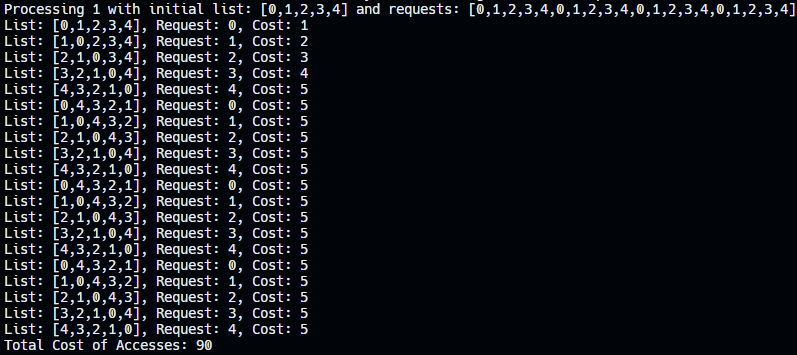
\includegraphics[width=15cm, height=7.5cm,]{images/1.png}}\\
\vspace{0.02in}
\small\textcolor{FSBlue}{Imagen 1: Costo total, lista de configuración, solicitud, y costo de cada elemento en la secuencia de solicitudes del Inciso 1 utilizando el algoritmo MTF.}
\end{center}

\subsection*{\textit{\textbf{Inciso 2}}}

\begin{center}
\fbox{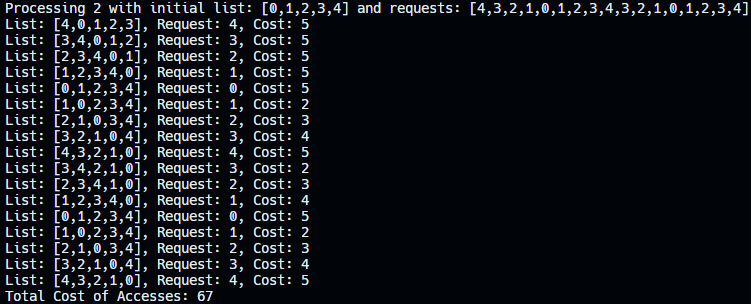
\includegraphics[width=15cm, height=7.5cm,]{images/2.png}}\\
\vspace{0.02in}
\small\textcolor{FSBlue}{Imagen 2: Costo total, lista de configuración, solicitud, y costo de cada elemento en la secuencia de solicitudes del Inciso 2 utilizando el algoritmo MTF.}
\end{center}

\subsection*{\textit{\textbf{Inciso 3}}}

Para la secuencia óptima de 20 solicitudes, se consideró acceder siempre al primer elemento de la lista (el elemento 0). Dado que este tiene el menor costo en cada solicitud, conduce al costo total más bajo.\\

\begin{center}
\fbox{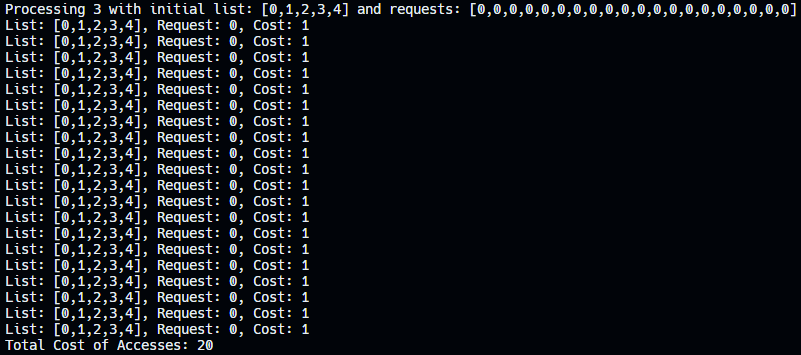
\includegraphics[width=15cm, height=7.5cm,]{images/3.png}}\\
\vspace{0.02in}
\small\textcolor{FSBlue}{Imagen 3: Costo total, lista de configuración, solicitud, y costo de cada elemento en la secuencia de solicitudes óptima utilizando el algoritmo MTF.}
\end{center}

\subsection*{\textit{\textbf{Inciso 4}}}

Para la secuencia de 20 solicitudes en el peor de los casos, se decidió acceder siempre al último elemento de la lista de configuración ya que este siempre tendrá el costo más alto. Esto se logra fácilmente generando una secuencia de solicitudes en la que los elementos de la lista de configuración se organizan de forma inversa\\

\begin{center}
\fbox{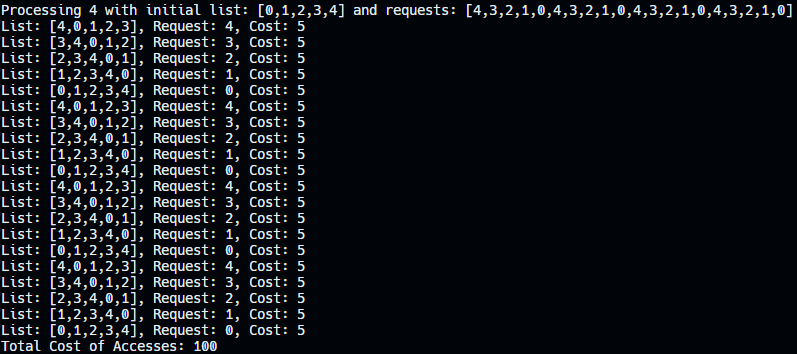
\includegraphics[width=15cm, height=7.5cm,]{images/4.png}}\\
\vspace{0.02in}
\small\textcolor{FSBlue}{Imagen 4: Costo total, lista de configuración, solicitud, y costo de cada elemento en la secuencia de solicitudes del peor caso utilizando el algoritmo MTF.}
\end{center}

\subsection*{\textit{\textbf{Inciso 5}}}

Al utilizar una secuencia de configuración \(n\), donde todos los elementos son iguales, sobre una lista de configuración \(m\), se puede observar un patrón a partir del cual se puede derivar una fórmula de costo total que evita ejecutar la secuencia completa y se enfoca solo en el primer elemento:

\[costoTotal = costo(n_{i}) + longitud(n) - 1\]

\begin{center}
\fbox{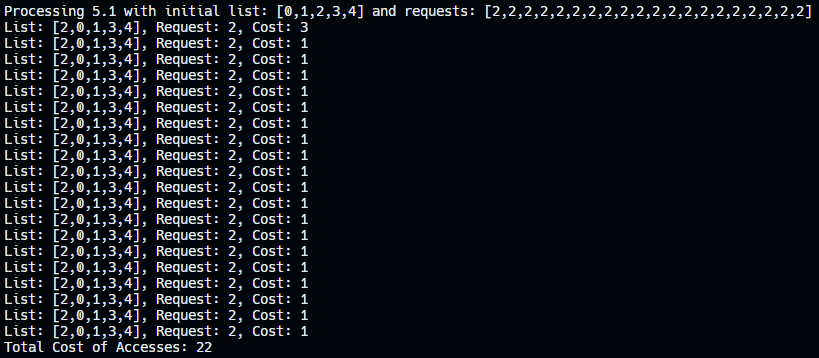
\includegraphics[width=15cm, height=7.5cm,]{images/5.1.png}}\\
\vspace{0.02in}
\small\textcolor{FSBlue}{Imagen 5.1: Costo total, lista de configuración, solicitud, y costo de cada elemento en la secuencia de solicitudes de 20 donde todos los elementos son 2 utilizando el algoritmo MTF.}
\end{center}

\begin{center}
\fbox{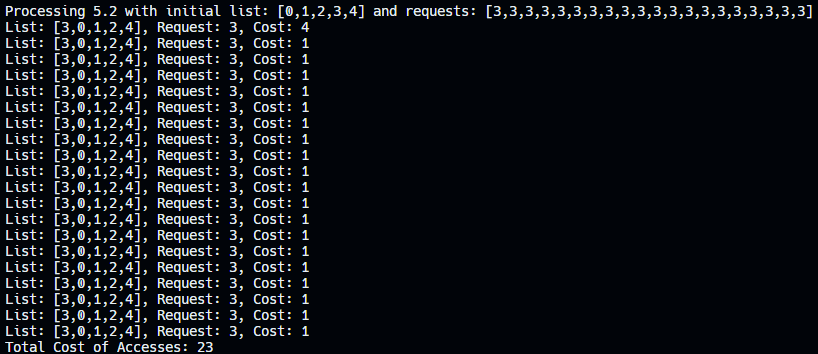
\includegraphics[width=15cm, height=7.5cm,]{images/5.2.png}}\\
\vspace{0.02in}
\small\textcolor{FSBlue}{Imagen 5.2: Costo total, lista de configuración, solicitud, y costo de cada elemento en la secuencia de solicitudes de 20 donde todos los elementos son 3 utilizando el algoritmo MTF.}
\end{center}

\subsection*{\textit{\textbf{Inciso 6}}}

\begin{center}
\fbox{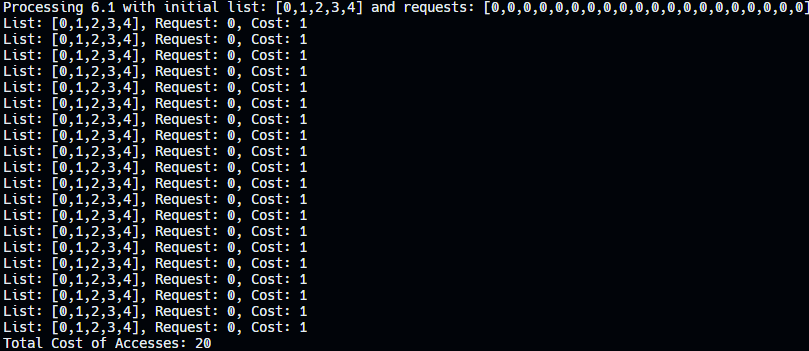
\includegraphics[width=15cm, height=7.5cm,]{images/6.1.png}}\\
\vspace{0.02in}
\small\textcolor{FSBlue}{Imagen 6.1: Costo total, lista de configuración, solicitud, y costo de cada elemento en la secuencia de solicitudes propuesta en el Inciso 3 (óptima) utilizando el algoritmo IMTF.}
\end{center}

\begin{center}
\fbox{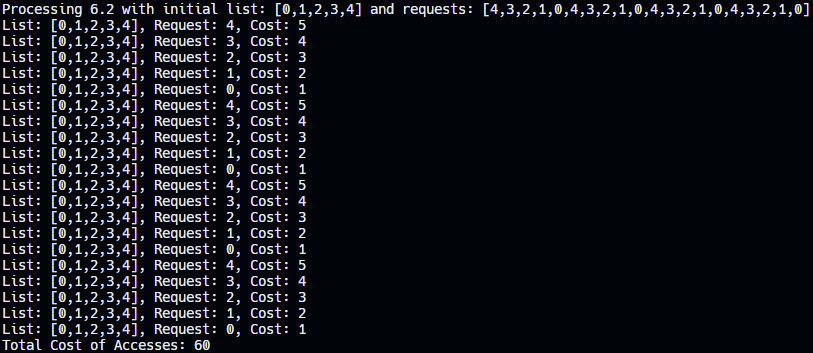
\includegraphics[width=15cm, height=7.5cm,]{images/6.2.png}}\\
\vspace{0.02in}
\small\textcolor{FSBlue}{Imagen 6.2: Costo total, lista de configuración, solicitud, y costo de cada elemento en la secuencia de solicitudes propuesta en el Inciso 4 (peor caso) utilizando el algoritmo IMTF.}
\end{center}
